\documentclass[aspectratio=169, 10pt]{beamer}

% --- Typography & Font Setup ---
\usepackage{fontspec}
\setmainfont{Arial}
\setsansfont{Arial}
\setmonofont{Consolas}[Scale=0.88]

\usefonttheme{professionalfonts}

% --- Color Palette ---
\usepackage{xcolor}
\definecolor{primaryblue}{RGB}{10, 47, 100}      % NEU Deep Navy
\definecolor{secondarygreen}{RGB}{0, 128, 128}   % Teal / Modern Tech Green
\definecolor{accentorange}{RGB}{217, 119, 6}     % Warm Amber
\definecolor{darkgray}{RGB}{45, 55, 72}
\definecolor{lightbg}{RGB}{247, 250, 252}
\definecolor{boxbg}{RGB}{240, 244, 248}
\definecolor{codebg}{RGB}{245, 245, 245}

% --- Theme Setup ---
\setbeamercolor{normal text}{fg=darkgray, bg=white}
\setbeamercolor{structure}{fg=primaryblue}
\setbeamercolor{frametitle}{fg=white, bg=primaryblue}
\setbeamercolor{title}{fg=white}
\setbeamercolor{subtitle}{fg=accentorange}
\setbeamercolor{item}{fg=secondarygreen}
\setbeamercolor{subitem}{fg=primaryblue}

% --- Tcolorbox Containers ---
\usepackage{tcolorbox}
\tcbuselibrary{skins}

\newtcolorbox{cbox}[2][primaryblue]{
  colback=#1!4,
  colframe=#1,
  coltitle=white,
  fonttitle=\bfseries\footnotesize,
  title={#2},
  arc=3pt,
  boxrule=0.9pt,
  left=4pt, right=4pt, top=3pt, bottom=3pt, boxsep=1pt,
  toptitle=1.5pt, bottomtitle=1.5pt,
  enhanced,
  drop fuzzy shadow=black!10
}

\newtcolorbox{promptbox}[1]{
  colback=lightbg,
  colframe=primaryblue!60,
  fonttitle=\bfseries\footnotesize,
  coltitle=primaryblue!90,
  title={#1},
  arc=3pt,
  boxrule=0.7pt,
  left=5pt, right=5pt, top=3pt, bottom=3pt, boxsep=1pt,
  enhanced
}

% --- TikZ Setup ---
\usepackage{tikz}
\usetikzlibrary{shapes.geometric, arrows.meta, positioning, calc, shadows}

% --- Tables & Code ---
\usepackage{booktabs}
\usepackage{tabularx}
\usepackage{listings}
\usepackage{xurl}

\lstset{
  backgroundcolor=\color{codebg},
  basicstyle=\ttfamily\scriptsize,
  breaklines=true,
  frame=single,
  rulecolor=\color{gray!30},
  keywordstyle=\color{primaryblue}\bfseries,
  commentstyle=\color{gray},
  stringstyle=\color{accentorange}
}

% --- Beamer Template Customization ---
\setbeamertemplate{navigation symbols}{}

\setbeamertemplate{frametitle}{%
  \nointerlineskip%
  \begin{beamercolorbox}[wd=\paperwidth,ht=3.2ex,dp=1.2ex,leftskip=0.5cm,rightskip=0.5cm]{frametitle}%
    \textbf{\insertframetitle}%
  \end{beamercolorbox}%
}

\setbeamertemplate{footline}{%
  \begin{beamercolorbox}[wd=\paperwidth,ht=2.4ex,dp=1.0ex,leftskip=0.5cm,rightskip=0.5cm]{author in head/foot}%
    \tiny\color{gray}%
    Dr. Vu Duc Minh (NEU) \hfill DSAI1003: Fundamental Programming Concepts in Python \hfill \insertframenumber{} / \inserttotalframenumber
  \end{beamercolorbox}%
}

% --- Metadata ---
\title{COURSE HANDBOOK \& SELF-STUDY GUIDE}
\subtitle{DSAI1003: FUNDAMENTAL PROGRAMMING CONCEPTS IN PYTHON}
\author{Dr. Vu Duc Minh}
\institute{Faculty of Data Science and AI -- School of Technology \\ National Economics University (NEU)}
\date{Semester I, Academic Year 2024 -- 2025}

\begin{document}

% ==============================================================================
% SLIDE 1: TITLE SLIDE
% ==============================================================================
\begin{frame}[plain]
  \vspace{0.2cm}
  \begin{tcolorbox}[colback=primaryblue, colframe=primaryblue, arc=4pt, left=12pt, right=12pt, top=10pt, bottom=10pt]
    \centering
    \textcolor{white}{\footnotesize\textbf{NATIONAL ECONOMICS UNIVERSITY -- SCHOOL OF TECHNOLOGY}}\\[1pt]
    \textcolor{white}{\scriptsize\textbf{FACULTY OF DATA SCIENCE AND ARTIFICIAL INTELLIGENCE}}\\[8pt]
    {\large\textbf{\textcolor{white}{COURSE HANDBOOK \& SELF-STUDY GUIDE}}}\\[3pt]
    {\large\textbf{\textcolor{accentorange}{DSAI1003: FUNDAMENTAL PROGRAMMING CONCEPTS IN PYTHON}}}\\[4pt]
    {\footnotesize\textcolor{white!80}{\textit{An Essential Foundation for Data Science \& AI}}}
  \end{tcolorbox}
  \vspace{0.15cm}
  \begin{tcolorbox}[colback=white, colframe=primaryblue!40, arc=3pt, left=8pt, right=8pt, top=5pt, bottom=5pt]
    \footnotesize
    \begin{tabularx}{\textwidth}{lX lX}
      \textbf{Instructor:} & Dr. Vu Duc Minh & \textbf{Program:} & Data Science in Finance \& E-commerce (DSFE) \\
      \textbf{Workload:} & 3 Credits (45h LT + 22.5h Lab) & \textbf{Decision:} & 975/QĐ-ĐHKTQD (30/03/2024) \\
      \textbf{Website:} & \url{https://vudmvn.github.io/Fundamental-of-Programming-Concepts-in-Python/} \\
    \end{tabularx}
  \end{tcolorbox}
\end{frame}

% ==============================================================================
% SLIDE 2: AGENDA
% ==============================================================================
\begin{frame}{Course Presentation Agenda}
  \begin{columns}[T]
    \begin{column}{0.49\textwidth}
      \begin{cbox}[primaryblue]{Part 1: Course Overview (Syllabus)}
        \footnotesize
        \begin{itemize}\setlength{\itemsep}{1pt}
          \item Course description \& pedagogical approach
          \item Learning objectives (COs G1 -- G7)
          \item International textbooks \& grading scheme
          \item 15-week detailed teaching schedule
        \end{itemize}
      \end{cbox}
      \vspace{0.1cm}
      \begin{cbox}[secondarygreen]{Part 2: Effective Self-Study Methods}
        \footnotesize
        \begin{itemize}\setlength{\itemsep}{1pt}
          \item 4 fatal pitfalls \& core principles
          \item The 9-step active study cycle
          \item Predict $\rightarrow$ Run $\rightarrow$ Explain \& Teach-Back
          \item 8-step debugging \& Personal Error Log
        \end{itemize}
      \end{cbox}
    \end{column}
    \begin{column}{0.49\textwidth}
      \begin{cbox}[accentorange]{Part 3: Leveraging AI for Breakthroughs}
        \footnotesize
        \begin{itemize}\setlength{\itemsep}{1pt}
          \item Positioning: AI Personal Tutor \& Coach
          \item 4-part structured prompt framework
          \item 5T Principle \& 3-level hint system
          \item Actionable Prompt Toolkit \& Verification
        \end{itemize}
      \end{cbox}
      \vspace{0.1cm}
      \begin{cbox}[darkgray]{Part 4: Week 1 Action Plan}
        \footnotesize
        \begin{itemize}\setlength{\itemsep}{1pt}
          \item Environment setup (VS Code, Colab)
          \item Explore GitHub course resources
          \item Initialize personal Learning Log
          \item Commit to active learning culture
        \end{itemize}
      \end{cbox}
    \end{column}
  \end{columns}
\end{frame}

% ==============================================================================
% PART 1: SYLLABUS
% ==============================================================================
\begin{frame}[plain]
  \vfill
  \begin{tcolorbox}[colback=primaryblue, colframe=primaryblue, arc=5pt, left=15pt, right=15pt, top=15pt, bottom=15pt]
    \textcolor{accentorange}{\large\textbf{PART 1}}\\[4pt]
    {\LARGE\textbf{\textcolor{white}{COURSE OVERVIEW (SYLLABUS)}}}\\[6pt]
    \textcolor{white!80}{\small Course Description, Objectives, Textbooks, Assessment \& 15-Week Roadmap}
  \end{tcolorbox}
  \vfill
\end{frame}

% SLIDE 4: Course Introduction & Philosophy
\begin{frame}{1. Course Description \& Pedagogical Approach}
  \begin{columns}[T]
    \begin{column}{0.49\textwidth}
      \begin{cbox}[primaryblue]{Curricular Position \& Audience}
        \small
        \begin{itemize}\setlength{\itemsep}{2pt}
          \item \textbf{Course Code:} DSAI1003 (3 Credits).
          \item \textbf{Target Audience:} Undergraduate students in \textit{Data Science in Finance \& E-commerce (DSFE)}.
          \item \textbf{Curricular Nature:} \textbf{Compulsory core foundation} establishing algorithmic mindset for advanced DS/AI studies.
        \end{itemize}
      \end{cbox}
    \end{column}
    \begin{column}{0.49\textwidth}
      \begin{cbox}[secondarygreen]{Pedagogical Philosophy}
        \small
        \begin{itemize}\setlength{\itemsep}{2pt}
          \item \textbf{No prior experience required:} Only standard high school algebra and logical reasoning needed.
          \item \textbf{Practical real-world focus:} Case studies in business, finance, retail analytics, and e-commerce.
          \item \textbf{Structured progression:} Algorithmic logic $\rightarrow$ Syntax $\rightarrow$ Built-in collections $\rightarrow$ OOP.
        \end{itemize}
      \end{cbox}
    \end{column}
  \end{columns}
  \vspace{0.12cm}
  \begin{tcolorbox}[colback=primaryblue!8, colframe=primaryblue!60, arc=3pt, left=8pt, right=8pt, top=3pt, bottom=3pt]
    \footnotesize
    \textbf{Learning Commitment:} Students will gain the competence to independently design and implement robust programs solving business analytics tasks, fully prepared for Machine Learning and AI courses.
  \end{tcolorbox}
\end{frame}

% SLIDE 5: Course Objectives (COs)
\begin{frame}{2. Course Objectives (Course Learning Outcomes)}
  \begin{columns}[T]
    \begin{column}{0.49\textwidth}
      \begin{cbox}[primaryblue]{Algorithmic Logic \& Core Syntax}
        \footnotesize
        \begin{itemize}\setlength{\itemsep}{3pt}
          \item \textbf{G1 (Algorithmic Thinking):} Express algorithms via pseudocode and flowcharts; implement console/GUI apps.
          \item \textbf{G2 (Python Foundations):} Master data types, expressions, decision branches, loops, and modular functions.
          \item \textbf{G3 (Data Collections):} Manage data efficiently using Lists, Tuples, Sets, and Dictionaries.
        \end{itemize}
      \end{cbox}
    \end{column}
    \begin{column}{0.49\textwidth}
      \begin{cbox}[secondarygreen]{Practical Applications \& DSFE Focus}
        \footnotesize
        \begin{itemize}\setlength{\itemsep}{3pt}
          \item \textbf{G4 (File I/O \& Exceptions):} Safe file operations (text/binary) and robust exception handling.
          \item \textbf{G5 (Object-Oriented Programming):} Model domain entities with Classes, Objects, and Inheritance.
          \item \textbf{G6 (Modern Developer Tools):} Proficient use of VS Code, Git, Google Colab, and AI assistants.
          \item \textbf{G7 (Applied Real-World Projects):} Solve end-to-end data processing tasks in business and finance.
        \end{itemize}
      \end{cbox}
    \end{column}
  \end{columns}
\end{frame}

% SLIDE 6: Textbooks & Evaluation
\begin{frame}{3. International Textbooks \& Grading Scheme}
  \begin{columns}[T]
    \begin{column}{0.49\textwidth}
      \begin{cbox}[primaryblue]{3 Standard International Textbooks}
        \footnotesize
        \begin{enumerate}\setlength{\itemsep}{3pt}
          \item \textbf{[1] Python for Everyone} (3rd Ed., 2019)\\
          \textit{Cay Horstmann, Rance Necaise} (Wiley)\\
          $\rightarrow$ \textbf{Main textbook} for syntax \& algorithmic design.
          \item \textbf{[2] Intro to Python for CS and Data Science} (2020)\\
          \textit{Paul Deitel, Harvey Deitel} (Pearson)\\
          $\rightarrow$ \textbf{Main textbook} for data processing \& AI.
          \item \textbf{[3] The Python Workbook} (2nd Ed., 2019)\\
          \textit{Ben Stephenson} (Springer)\\
          $\rightarrow$ Self-study exercises with complete solutions.
        \end{enumerate}
      \end{cbox}
    \end{column}
    \begin{column}{0.49\textwidth}
      \begin{cbox}[secondarygreen]{Assessment Components (3 Grades)}
        \scriptsize
        \begin{tabularx}{\textwidth}{lX c}
          \toprule
          \textbf{Component} & \textbf{Scope \& Criteria} & \textbf{Weight} \\
          \midrule
          \textbf{Homework (HW)} & Theory \& coding (LMS, bi-weekly) & \textbf{30\%} \\
          \textbf{Midterm Exam} & Week 7 exam (Lessons 1 -- 6) & \textbf{30\%} \\
          \textbf{Final Exam} & Computer lab practical test (Week 15) & \textbf{40\%} \\
          \bottomrule
        \end{tabularx}
      \end{cbox}
      \vspace{0.1cm}
      \begin{cbox}[accentorange]{Academic Regulations}
        \footnotesize
        \begin{itemize}\setlength{\itemsep}{2pt}
          \item \textbf{Attendance:} Minimum \textbf{80\%} class attendance required.
          \item \textbf{Passing grade:} Final composite grade $\ge$ \textbf{5.0 / 10.0}.
        \end{itemize}
      \end{cbox}
    \end{column}
  \end{columns}
\end{frame}

% SLIDE 7: 15-week Roadmap Phase 1
\begin{frame}{4. 15-Week Teaching Plan -- Phase 1 (Weeks 1 -- 7)}
  \scriptsize
  \begin{tabularx}{\textwidth}{c l X l}
    \toprule
    \textbf{Week} & \textbf{Lesson \& Topic} & \textbf{Core Knowledge Focus} & \textbf{Assessment} \\
    \midrule
    \textbf{1} & \textbf{Lesson 1: Intro \& Algorithms} & Computers, Python interpreter, pseudocode, flowcharts & Environment setup \\
    \textbf{2} & \textbf{Lesson 2: Software Process \& Types} & Numbers, strings, assignments, variables, modules & \textbf{Homework \#1} \\
    \textbf{3} & \textbf{Lesson 3: Decision Structures} & Branching \texttt{if}, \texttt{if-else}, \texttt{if-elif-else}, Boolean & Due: HW \#1 \\
    \textbf{4} & \textbf{Lesson 4: Loop Structures} & Loops \texttt{while}, \texttt{for}, nested loops, strings & \textbf{Homework \#2} \\
    \textbf{5} & \textbf{Lesson 5: Function Design} & Syntax \texttt{def}, parameters, return, scope & Due: HW \#2 \\
    \textbf{6} & \textbf{Lesson 6: Lists \& Tuples} & 1D/2D arrays, slicing, built-in methods & \textbf{Homework \#3} \\
    \textbf{7} & \textbf{Midterm Examination} & Synthesis \& assessment of Lessons 1 -- 6 & \textbf{Midterm (30\%)} \\
    \bottomrule
  \end{tabularx}
\end{frame}

% SLIDE 8: 15-week Roadmap Phase 2
\begin{frame}{5. 15-Week Teaching Plan -- Phase 2 (Weeks 8 -- 15)}
  \scriptsize
  \begin{tabularx}{\textwidth}{c l X l}
    \toprule
    \textbf{Week} & \textbf{Lesson \& Topic} & \textbf{Core Knowledge Focus} & \textbf{Assessment} \\
    \midrule
    \textbf{8--9} & \textbf{Lesson 7: File I/O \& Exceptions} & Text file reading/writing, \texttt{sys.argv}, \texttt{try-except} & \textbf{Homework \#4} \\
    \textbf{10} & \textbf{Lesson 8: Sets \& Dictionaries} & Key-value mappings, hash tables, nested JSON records & E-commerce case study \\
    \textbf{11--12} & \textbf{Lesson 9: Objects \& Classes (OOP 1)} & OOP mindset, \texttt{class}, \texttt{\_\_init\_\_}, methods & Mini-lab OOP \\
    \textbf{13--14} & \textbf{Lesson 10: Inheritance \& Polymorphism} & Inheritance hierarchy, \texttt{super()}, method overriding & Final exam review \\
    \textbf{15} & \textbf{Course Review \& Exam Prep} & Comprehensive synthesis of all course topics & Mock lab test \\
    \bottomrule
  \end{tabularx}
\end{frame}

% ==============================================================================
% PART 2: EFFECTIVE SELF-STUDY METHODOLOGY
% ==============================================================================
\begin{frame}[plain]
  \vfill
  \begin{tcolorbox}[colback=secondarygreen, colframe=secondarygreen, arc=5pt, left=15pt, right=15pt, top=15pt, bottom=15pt]
    \textcolor{white}{\large\textbf{PART 2}}\\[4pt]
    {\LARGE\textbf{\textcolor{white}{EFFECTIVE PYTHON SELF-STUDY METHODS}}}\\[6pt]
    \textcolor{white!80}{\small Overcoming Pitfalls, 9-Step Study Cycle, Active Learning \& Systematic Debugging}
  \end{tcolorbox}
  \vfill
\end{frame}

% SLIDE 10: Core Principle & 4 Pitfalls
\begin{frame}{6. The Nature of Programming \& 4 Fatal Pitfalls}
  \begin{tcolorbox}[colback=accentorange!12, colframe=accentorange, arc=3pt, left=6pt, right=6pt, top=2.5pt, bottom=2.5pt]
    \centering\footnotesize\bfseries
    "Learn programming by reading less, practicing more, and thinking before looking at solutions."
  \end{tcolorbox}
  \vspace{0.06cm}
  \begin{columns}[T]
    \begin{column}{0.49\textwidth}
      \begin{cbox}[accentorange]{Pitfall 1: Reading without running code}
        \scriptsize
        Skimming sample code and assuming understanding. When the screen is off, cannot reproduce a single line.
      \end{cbox}
      \vspace{0.06cm}
      \begin{cbox}[accentorange]{Pitfall 2: Blind copy-pasting}
        \scriptsize
        Copying code from the web or AI; code executes, but the learner cannot explain why specific statements exist.
      \end{cbox}
    \end{column}
    \begin{column}{0.49\textwidth}
      \begin{cbox}[accentorange]{Pitfall 3: Checking solutions prematurely}
        \scriptsize
        Opening solutions immediately when stuck. Bypasses the productive cognitive struggle where problem-solving develops.
      \end{cbox}
      \vspace{0.06cm}
      \begin{cbox}[accentorange]{Pitfall 4: Cramming too many topics}
        \scriptsize
        Rushing from variables to OOP in 2 days without allowing time for concepts to consolidate through practice.
      \end{cbox}
    \end{column}
  \end{columns}
\end{frame}

% SLIDE 11: 9-Step Active Study Cycle
\begin{frame}{7. The 9-Step Active Programming Study Cycle}
  \begin{center}
  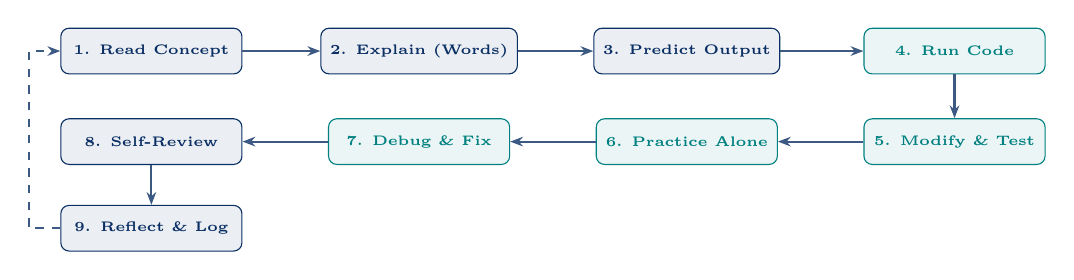
\begin{tikzpicture}[
      stepb/.style={rectangle, rounded corners=3pt, draw=primaryblue, fill=primaryblue!8, text=primaryblue, font=\tiny\bfseries, minimum height=0.58cm, minimum width=2.3cm, align=center},
      stepg/.style={rectangle, rounded corners=3pt, draw=secondarygreen, fill=secondarygreen!8, text=secondarygreen, font=\tiny\bfseries, minimum height=0.58cm, minimum width=2.3cm, align=center},
      arr/.style={-{Stealth[scale=0.7]}, thick, primaryblue!80}
  ]
    % Row 1
    \node[stepb] (s1) at (0.6, 1.8) {1. Read Concept};
    \node[stepb] (s2) at (4.0, 1.8) {2. Explain (Words)};
    \node[stepb] (s3) at (7.4, 1.8) {3. Predict Output};
    \node[stepg] (s4) at (10.8, 1.8) {4. Run Code};

    % Row 2
    \node[stepg] (s5) at (10.8, 0.65) {5. Modify \& Test};
    \node[stepg] (s6) at (7.4, 0.65) {6. Practice Alone};
    \node[stepg] (s7) at (4.0, 0.65) {7. Debug \& Fix};
    \node[stepb] (s8) at (0.6, 0.65) {8. Self-Review};

    % Step 9
    \node[stepb] (s9) at (0.6, -0.45) {9. Reflect \& Log};

    % Connections
    \draw[arr] (s1) -- (s2); \draw[arr] (s2) -- (s3); \draw[arr] (s3) -- (s4);
    \draw[arr] (s4) -- (s5);
    \draw[arr] (s5) -- (s6); \draw[arr] (s6) -- (s7); \draw[arr] (s7) -- (s8);
    \draw[arr] (s8) -- (s9);
    \draw[arr, dashed] (s9.west) -- ++(-0.4, 0) |- (s1.west);
  \end{tikzpicture}
  \end{center}
  \vspace{0.05cm}
  \begin{tcolorbox}[colback=secondarygreen!8, colframe=secondarygreen, arc=3pt, left=8pt, right=8pt, top=3pt, bottom=3pt]
    \textbf{\footnotesize The 70/30 Golden Rule of Self-Study:} \\
    \footnotesize Allocate at most \textbf{30\% of study time} to reading theory; dedicate over \textbf{70\% of time} directly to hands-on coding: typing, observing runtime errors, analyzing tracebacks, and solving unassisted problems!
  \end{tcolorbox}
\end{frame}

% SLIDE 12: Active Learning Techniques
\begin{frame}{8. Breakthrough Active Learning Techniques}
  \begin{columns}[T]
    \begin{column}{0.49\textwidth}
      \begin{cbox}[primaryblue]{Predict $\rightarrow$ Run $\rightarrow$ Explain}
        \footnotesize
        \textbf{Before clicking Run on the IDE:}
        \begin{itemize}\setlength{\itemsep}{1.5pt}
          \item Write down exact expected terminal output.
          \item Predict how memory and variables change state.
          \item If output differs $\rightarrow$ That is where maximum learning occurs!
        \end{itemize}
      \end{cbox}
      \vspace{0.06cm}
      \begin{cbox}[secondarygreen]{Teach-Back Technique}
        \footnotesize
        Explain concepts to a beginner in simple terms. Saying \textit{"It works because it has to"} proves you do not truly understand the mechanism!
      \end{cbox}
    \end{column}
    \begin{column}{0.49\textwidth}
      \begin{cbox}[accentorange]{Active Recall (Self-Testing)}
        \footnotesize
        \textbf{Do not repeatedly reread slides!}
        \begin{itemize}\setlength{\itemsep}{1.5pt}
          \item Close notes and answer diagnostic checks:
          \begin{itemize}\scriptsize
            \item What type does \texttt{input()} return?
            \item How do you cast to an integer?
            \item Why does string + integer cause an error?
          \end{itemize}
        \end{itemize}
      \end{cbox}
      \vspace{0.06cm}
      \begin{cbox}[darkgray]{Spaced Repetition Schedule}
        \footnotesize
        Review on an expanding interval:\\
        \centering\textbf{Day 1 $\rightarrow$ Day 3 $\rightarrow$ Day 7 $\rightarrow$ Day 14}\\
        \raggedright Converts short-term memory into lasting intuition.
      \end{cbox}
    \end{column}
  \end{columns}
\end{frame}

% SLIDE 13: The 5-Level Learning Ladder
\begin{frame}{9. The 5-Level Learning Ladder}
  \begin{center}
  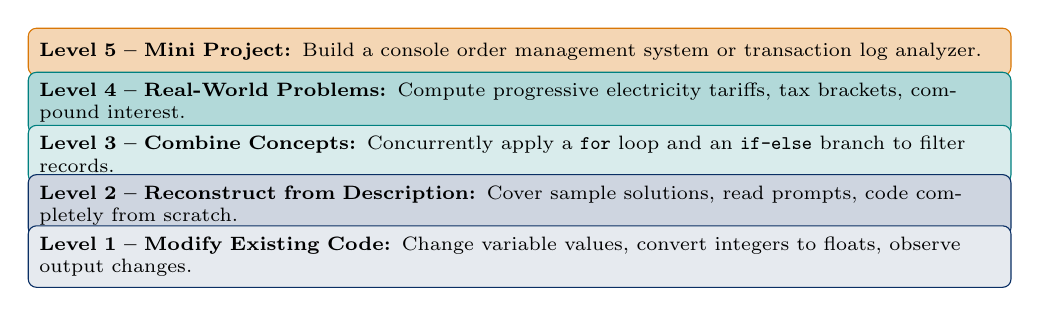
\begin{tikzpicture}[
    ladder/.style={rectangle, rounded corners=3pt, text width=12.2cm, minimum height=0.60cm, inner sep=4pt, font=\scriptsize, align=left}
  ]
    \node[ladder, fill=accentorange!30, draw=accentorange] at (0, 2.6) {\textbf{Level 5 -- Mini Project:} Build a console order management system or transaction log analyzer.};
    \node[ladder, fill=secondarygreen!30, draw=secondarygreen] at (0, 1.95) {\textbf{Level 4 -- Real-World Problems:} Compute progressive electricity tariffs, tax brackets, compound interest.};
    \node[ladder, fill=secondarygreen!15, draw=secondarygreen] at (0, 1.3) {\textbf{Level 3 -- Combine Concepts:} Concurrently apply a \texttt{for} loop and an \texttt{if-else} branch to filter records.};
    \node[ladder, fill=primaryblue!20, draw=primaryblue] at (0, 0.65) {\textbf{Level 2 -- Reconstruct from Description:} Cover sample solutions, read prompts, code completely from scratch.};
    \node[ladder, fill=primaryblue!10, draw=primaryblue] at (0, 0) {\textbf{Level 1 -- Modify Existing Code:} Change variable values, convert integers to floats, observe output changes.};
  \end{tikzpicture}
  \end{center}
  \vspace{0.1cm}
  \centering\small\itshape
  Never leap directly from basic examples to complex projects without ascending each intermediate ladder rung!
\end{frame}

% SLIDE 14: Debugging Framework
\begin{frame}{10. Debugging Skills \& Standard Error Classification}
  \begin{columns}[T]
    \begin{column}{0.49\textwidth}
      \begin{cbox}[primaryblue]{Standard 8-Step Debugging Protocol}
        \scriptsize
        \begin{enumerate}\setlength{\itemsep}{1.5pt}
          \item Read the traceback from the bottom line upward.
          \item Pinpoint the exact file and line number.
          \item Identify the error type (\texttt{TypeError}, \texttt{IndexError}...).
          \item Insert \texttt{print()} statements to inspect variables.
          \item Use \texttt{type()} to verify runtime data types.
          \item Compare observed output against expectations.
          \item Test against minimal, simplified input sets.
          \item \textbf{Change only 1 element} between test runs!
        \end{enumerate}
      \end{cbox}
    \end{column}
    \begin{column}{0.49\textwidth}
      \begin{cbox}[accentorange]{Distinguishing 3 Error Categories}
        \footnotesize
        \begin{itemize}\setlength{\itemsep}{3pt}
          \item \textbf{Syntax Error:} Violating language grammar (missing \texttt{:}, unmatched parentheses). Caught immediately upon loading.
          \item \textbf{Runtime Error:} Valid syntax that crashes during execution (division by zero, invalid type casting).
          \item \textbf{Logic Error:} Program runs without errors but \textbf{produces incorrect calculations}! (Most dangerous).
        \end{itemize}
      \end{cbox}
    \end{column}
  \end{columns}
\end{frame}

% SLIDE 15: Error Log
\begin{frame}{11. Personal Learning Log \& Error Tracking (Error Log)}
  \begin{tcolorbox}[colback=secondarygreen!8, colframe=secondarygreen, arc=3pt, left=8pt, right=8pt, top=3pt, bottom=3pt]
    \textbf{\footnotesize Transforming Mistakes into Intellectual Assets:} \\
    \footnotesize Documenting encountered errors systematically converts painful bugs into invaluable personal mastery that prevents exam errors.
  \end{tcolorbox}
  \vspace{0.1cm}
  \scriptsize
  \begin{tabularx}{\textwidth}{l X X c}
    \toprule
    \textbf{Error Message} & \textbf{Root Cause} & \textbf{Correction Strategy} & \textbf{Clear?} \\
    \midrule
    \texttt{TypeError: can only} & \texttt{input()} always returns a string (\texttt{str}), & Explicitly cast: \texttt{int(input())} or & $\checkmark$ \\
    \texttt{concatenate str to str} & which cannot be added to numbers. & \texttt{float(input())}. & \\
    \midrule
    \texttt{IndexError: list index} & Valid indices range from $0$ to $N-1$; accessing & Fix iteration boundaries: & $\checkmark$ \\
    \texttt{out of range} & index $N$ causes out-of-bounds error. & \texttt{range(len(lst))}. & \\
    \midrule
    Infinite loop (\texttt{while}) & Forgot to increment step variable in loop body. & Add statement: \texttt{i += 1}. & $\checkmark$ \\
    \bottomrule
  \end{tabularx}
  \vspace{0.15cm}
  \centering\footnotesize\itshape
  Maintain your \texttt{learning\_log.md} file after each study session to monitor weekly growth!
\end{frame}

% ==============================================================================
% PART 3: LEARNING PYTHON WITH AI
% ==============================================================================
\begin{frame}[plain]
  \vfill
  \begin{tcolorbox}[colback=accentorange, colframe=accentorange, arc=5pt, left=15pt, right=15pt, top=15pt, bottom=15pt]
    \textcolor{primaryblue}{\large\textbf{PART 3}}\\[4pt]
    {\LARGE\textbf{\textcolor{white}{STRATEGIC AI (CHATGPT) ASSISTED LEARNING}}}\\[6pt]
    \textcolor{white!90}{\small AI Tutor, 4-Part Prompt, 5T Principle, Prompt Toolkit \& Verification}
  \end{tcolorbox}
  \vfill
\end{frame}

% SLIDE 17: AI Positioning (Tutor vs. Crutch)
\begin{frame}{12. Positioning AI Accurately in Programming Education}
  \begin{columns}[T]
    \begin{column}{0.49\textwidth}
      \begin{cbox}[accentorange]{WARNING: Harmful Over-Reliance}
        \footnotesize
        \textbf{Flawed Workflow:}\\
        Prompt $\rightarrow$ Delegate to AI $\rightarrow$ Copy code $\rightarrow$ Paralysis!
        \vspace{2pt}
        \begin{itemize}\setlength{\itemsep}{2pt}
          \item Zero understanding of why statements are chosen.
          \item Completely helpless in proctored exam rooms without AI.
          \item Analytical problem-solving ability atrophies over time.
        \end{itemize}
      \end{cbox}
    \end{column}
    \begin{column}{0.49\textwidth}
      \begin{cbox}[secondarygreen]{RECOMMENDED: AI as Personal Coach}
        \footnotesize
        \textbf{Best-Practice Workflow:}\\
        Think $\rightarrow$ Draft code $\rightarrow$ Request hints $\rightarrow$ Code!
        \vspace{2pt}
        \begin{itemize}\setlength{\itemsep}{2pt}
          \item Ask AI to \textbf{explain} difficult concepts in plain terms.
          \item Request \textbf{incremental hints} without full solutions.
          \item Ask AI to \textbf{quiz your understanding} interactively.
          \item Request \textbf{code reviews} on your own hand-written code.
        \end{itemize}
      \end{cbox}
    \end{column}
  \end{columns}
\end{frame}

% SLIDE 18: 4-Part Prompt Framework
\begin{frame}{13. The 4-Part Structured Prompt Framework}
  \scriptsize
  \begin{tabularx}{\textwidth}{l p{3.2cm} X}
    \toprule
    \textbf{Component} & \textbf{Guiding Question} & \textbf{Practical Concrete Example} \\
    \midrule
    \textbf{1. Context} & Who are you, what level? & \textit{"I am a first-year student beginning foundational Python programming..."} \\
    \textbf{2. Problem} & Where are you stuck? & \textit{"I struggle to differentiate between variables and assigned values..."} \\
    \textbf{3. Task} & What should AI do? & \textit{"Explain with an everyday analogy and a Python snippet under 8 lines..."} \\
    \textbf{4. Constraint} & Boundaries on the response? & \textit{"Do not use functions or OOP; ask me 2 check questions without answers yet."} \\
    \bottomrule
  \end{tabularx}
  \vspace{0.15cm}
  \begin{tcolorbox}[colback=secondarygreen!8, colframe=secondarygreen, arc=3pt, left=8pt, right=8pt, top=3pt, bottom=3pt]
    \textbf{\footnotesize The Key Difference:}\\
    \footnotesize Compared to blunt queries like \textit{"What is a variable in Python?"}, structured prompts allow AI to tailor explanations precisely to your current knowledge level!
  \end{tcolorbox}
\end{frame}

% SLIDE 19: The 5T Principle
\begin{frame}{14. The 5T Principle for AI-Assisted Study}
  \begin{center}
  
\begin{tikzpicture}[
    tbox/.style={rectangle, rounded corners=4pt, draw=primaryblue, fill=primaryblue!6, text=primaryblue, minimum height=0.9cm, minimum width=2.0cm, align=center, font=\scriptsize\bfseries},
    arr/.style={-{Stealth[scale=0.7]}, thick, secondarygreen}
  ]
    \node[tbox] (t1) at (0, 0) {1. Think\\[1pt]\tiny\mdseries Independent mind};
    \node[tbox] (t2) at (2.6, 0) {2. Try\\[1pt]\tiny\mdseries Initial code draft};
    \node[tbox] (t3) at (5.2, 0) {3. Talk\\[1pt]\tiny\mdseries Targeted question};
    \node[tbox, draw=primaryblue!90, fill=primaryblue!15] (t4) at (7.8, 0) {4. Test\\[1pt]\tiny\mdseries Machine validation};
    \node[tbox] (t5) at (10.4, 0) {5. Teach-back\\[1pt]\tiny\mdseries Synthesize in words};

    \draw[arr] (t1) -- (t2);
    \draw[arr] (t2) -- (t3);
    \draw[arr] (t3) -- (t4);
    \draw[arr] (t4) -- (t5);
  \end{tikzpicture}
  \end{center}
  \vspace{0.05cm}
  \begin{columns}[T]
    \begin{column}{0.49\textwidth}
      \footnotesize
      \begin{itemize}\setlength{\itemsep}{2pt}
        \item \textbf{Think:} Formulate Inputs, Outputs, and algorithms before opening AI chat.
        \item \textbf{Try:} Type your first draft independently, even with bugs.
        \item \textbf{Talk:} Provide existing code and ask about the exact bottleneck.
      \end{itemize}
    \end{column}
    \begin{column}{0.49\textwidth}
      \footnotesize
      \begin{itemize}\setlength{\itemsep}{2pt}
        \item \textbf{Test:} Always run code on IDE; test edge cases (0, negatives, empty lists).
        \item \textbf{Teach-back:} Close chat window and explain the solution in your own words.
      \end{itemize}
    \end{column}
  \end{columns}
\end{frame}

% SLIDE 20: 3-Level Hint System
\begin{frame}{15. The Three-Level Hint System}
  \begin{tcolorbox}[colback=primaryblue!8, colframe=primaryblue, arc=3pt, left=6pt, right=6pt, top=2pt, bottom=2pt]
    \centering\footnotesize\bfseries When tackling difficult exercises, request tiered hints -- Never ask for complete solutions!
  \end{tcolorbox}
  \vspace{0.08cm}
  \begin{columns}[T]
    \begin{column}{0.32\textwidth}
      \begin{cbox}[primaryblue]{Level 1: Idea Hint}
        \scriptsize
        \textbf{(Conceptual Direction)}\\[2pt]
        Analyzes the problem and outlines mathematical/algorithmic logic.\\
        \vspace{2pt}
        $\rightarrow$ \textbf{Strictly zero lines of code provided!}
      \end{cbox}
    \end{column}
    \begin{column}{0.32\textwidth}
      \begin{cbox}[secondarygreen]{Level 2: Structure Hint}
        \scriptsize
        \textbf{(Architectural Clues)}\\[2pt]
        Suggests key statements: \texttt{for} loops, nested \texttt{if}, modulo operator \texttt{\%}...\\
        \vspace{2pt}
        $\rightarrow$ \textbf{Shapes the logic scaffold.}
      \end{cbox}
    \end{column}
    \begin{column}{0.32\textwidth}
      \begin{cbox}[accentorange]{Level 3: Scaffold Hint}
        \scriptsize
        \textbf{(Skeleton Template)}\\[2pt]
        Provides template code with blank placeholders (\texttt{\# TODO}) to implement.\\
        \vspace{2pt}
        $\rightarrow$ \textbf{Preserves intellectual ownership.}
      \end{cbox}
    \end{column}
  \end{columns}
  \vspace{0.1cm}
  \begin{tcolorbox}[colback=accentorange!10, colframe=accentorange, arc=3pt, left=6pt, right=6pt, top=2pt, bottom=2pt]
    \centering\scriptsize\bfseries
    Problem-Solving Strategy: Strive to solve problems using Level 1 hints. Only unlock Levels 2 and 3 after 15 minutes of unassisted effort!
  \end{tcolorbox}
\end{frame}

% SLIDE 21: Prompt Toolkit 1
\begin{frame}{16. Actionable Prompt Toolkit (1): Concepts \& Hints}
  \begin{columns}[T]
    \begin{column}{0.49\textwidth}
      \begin{cbox}[primaryblue]{New Concept (Concept Prompt)}
        \scriptsize
        I am a beginner learning Python. Please explain the concept of [Recursive Functions].\\[2pt]
        \textbf{Requirements:}
        \begin{enumerate}\setlength{\itemsep}{1pt}
          \item Intuitive explanation with 1 real-world analogy.
          \item Short code example (under 10 lines).
          \item 1 common pitfall beginners frequently make.
          \item 2 check questions without answers yet.
        \end{enumerate}
      \end{cbox}
    \end{column}
    \begin{column}{0.49\textwidth}
      \begin{cbox}[secondarygreen]{Exercise Hint (Socratic Hint)}
        \scriptsize
        I am solving this exercise: "[PROBLEM DESCRIPTION]"\\[2pt]
        My current code attempt:\\
        \texttt{[PASTE YOUR CODE HERE]}\\[2pt]
        I am blocked at step [DESCRIBE BOTTLENECK].\\[2pt]
        \textbf{Requirement:} ABSOLUTELY DO NOT write code for me. Give me a LEVEL 1 HINT regarding algorithmic ideas so I can think through it.
      \end{cbox}
    \end{column}
  \end{columns}
\end{frame}

% SLIDE 22: Prompt Toolkit 2
\begin{frame}{17. Actionable Prompt Toolkit (2): Debug \& Code Review}
  \begin{columns}[T]
    \begin{column}{0.49\textwidth}
      \begin{cbox}[accentorange]{Debugging Support (Root Cause)}
        \scriptsize
        I wrote Python code to achieve: [CODE OBJECTIVE]\\[2pt]
        Current code: \texttt{[PASTE CODE]}\\[2pt]
        Encountered error: \texttt{[PASTE TRACEBACK]}\\[2pt]
        \textbf{Requirements:}
        \begin{enumerate}\setlength{\itemsep}{1pt}
          \item Explain the root cause of this error.
          \item Point out the problematic line(s).
          \item Ask 1 guiding question so I can fix it myself; DO NOT rewrite my code.
        \end{enumerate}
      \end{cbox}
    \end{column}
    \begin{column}{0.49\textwidth}
      \begin{cbox}[primaryblue]{Code Review \& Optimization}
        \scriptsize
        I completed this exercise and code executes correctly: \texttt{[PASTE WORKING CODE]}\\[2pt]
        Act as an experienced Python Instructor:
        \begin{enumerate}\setlength{\itemsep}{1pt}
          \item Evaluate variable naming, readability, logic structure.
          \item Does the code handle edge cases safely?
          \item Suggest 1 concrete Pythonic optimization and explain why.
        \end{enumerate}
      \end{cbox}
    \end{column}
  \end{columns}
\end{frame}

% SLIDE 23: Prompt Toolkit 3
\begin{frame}{18. Actionable Prompt Toolkit (3): Self-Quiz Generation}
  \begin{cbox}[primaryblue]{Generating Practice Quizzes (Self-Quiz Prompt)}
    \footnotesize
    I just finished studying: \textbf{[Lists, Tuples, Slicing, and for Loops]}.\\[3pt]
    Create a 6-question diagnostic quiz for me:
    \begin{itemize}\setlength{\itemsep}{2pt}
      \item \textbf{2 Multiple-Choice:} 4 options A, B, C, D (exactly 1 correct answer).
      \item \textbf{2 Predict the Output:} Code snippet 3--5 lines using foundational features only.
      \item \textbf{2 Find the Bug:} Code snippet containing exactly 1 bug to identify and fix.
    \end{itemize}
    \vspace{2pt}
    \textbf{Constraint:} DO NOT show answers upfront. Wait for my submitted answers before grading and providing explanations!
  \end{cbox}
  \vspace{0.15cm}
  \begin{tcolorbox}[colback=secondarygreen!8, colframe=secondarygreen, arc=3pt, left=8pt, right=8pt, top=3pt, bottom=3pt]
    \textbf{\footnotesize Advanced Pro-Tip: Quizzes from Past Mistakes}\\
    \footnotesize Copy past error entries from your \texttt{learning\_log.md} into the prompt: \textit{"Create 5 quiz questions specifically targeting these past bugs to test whether I have truly overcome them!"}
  \end{tcolorbox}
\end{frame}

% SLIDE 24: 7-Point AI Verification Checklist
\begin{frame}{19. 7-Point AI-Generated Code Verification Checklist}
  \begin{columns}[T]
    \begin{column}{0.49\textwidth}
      \footnotesize
      \begin{itemize}\setlength{\itemsep}{3pt}
        \item[$\square$] \textbf{1. Curriculum Match:} Does the code avoid external libraries or advanced concepts beyond syllabus?
        \item[$\square$] \textbf{2. Practical Run:} Have you run the code in IDE without compilation/runtime errors?
        \item[$\square$] \textbf{3. Exact Spec Match:} Does output match problem requirements down to exact formatting?
        \item[$\square$] \textbf{4. Boundary Testing:} Does code handle edge cases (0, negatives, empty lists)?
      \end{itemize}
    \end{column}
    \begin{column}{0.49\textwidth}
      \footnotesize
      \begin{itemize}\setlength{\itemsep}{3pt}
        \item[$\square$] \textbf{5. Standard Terms:} Are terms aligned with official textbook (\textit{Python for Everyone})?
        \item[$\square$] \textbf{6. Line-by-Line Explanation:} Can you point to every line and explain why it exists?
        \item[$\square$] \textbf{7. Independent Reproduction:} Can you rewrite this code in 10 minutes without AI?
      \end{itemize}
    \end{column}
  \end{columns}
  \vspace{0.15cm}
  \begin{tcolorbox}[colback=accentorange!15, colframe=accentorange, arc=3pt, left=8pt, right=8pt, top=3pt, bottom=3pt]
    \centering\footnotesize
    \textbf{The Inviolable Golden Rule:}\\[2pt]
    \textbf{"NEVER SUBMIT OR PRESERVE SOURCE CODE\\THAT YOU CANNOT THOROUGHLY EXPLAIN YOURSELF!"}
  \end{tcolorbox}
\end{frame}

% ==============================================================================
% PART 4: ACTION PLAN FOR WEEK 1 & CONCLUSION
% ==============================================================================
\begin{frame}{20. Immediate Action Plan for Week 1}
  \begin{columns}[T]
    \begin{column}{0.32\textwidth}
      \begin{cbox}[primaryblue]{1. Environment Setup}
        \scriptsize
        \begin{itemize}\setlength{\itemsep}{2pt}
          \item Install \textbf{Python 3.11+} from \url{python.org}.
          \item Install \textbf{VS Code} editor with official Python extension pack.
          \item Set up a \textbf{Google Colab} account in your browser for instant coding.
        \end{itemize}
      \end{cbox}
    \end{column}
    \begin{column}{0.32\textwidth}
      \begin{cbox}[secondarygreen]{2. Resource Exploration}
        \scriptsize
        \begin{itemize}\setlength{\itemsep}{2pt}
          \item Bookmark course GitHub repo: \url{github.com/vudmvn/Python}.
          \item Read the detailed syllabus (\texttt{syllabus-en.md}).
          \item Read Chapter 1 of textbook \textit{Python for Everyone}.
        \end{itemize}
      \end{cbox}
    \end{column}
    \begin{column}{0.32\textwidth}
      \begin{cbox}[accentorange]{3. Self-Study Log}
        \scriptsize
        \begin{itemize}\setlength{\itemsep}{2pt}
          \item Create study folder \texttt{DSAI1003\_Python/} on machine.
          \item Create file \texttt{learning\_log.md} to log weekly progress.
          \item Save the Prompt Toolkit to interact with AI ethically and smartly.
        \end{itemize}
      \end{cbox}
    \end{column}
  \end{columns}
  \vspace{0.2cm}
  \begin{tcolorbox}[colback=primaryblue!5, colframe=primaryblue, arc=3pt, left=8pt, right=8pt, top=6pt, bottom=6pt]
    \centering\small
    \textbf{\textcolor{primaryblue}{WISHING ALL DATA SCIENCE \& AI STUDENTS}}\\[3pt]
    \textbf{\textcolor{secondarygreen}{MASTERY OF COMPUTATIONAL THINKING \& BREAKTHROUGH CAPABILITIES WITH AI!}}
  \end{tcolorbox}
\end{frame}

% SLIDE 26: THANK YOU
\begin{frame}[plain]
  \vfill
  \centering
  {\Huge\textbf{\textcolor{primaryblue}{THANK YOU!}}}\\[8pt]
  {\Large\textbf{\textcolor{secondarygreen}{FOR YOUR ATTENTION \& ENGAGEMENT}}}\\[15pt]

  \begin{tcolorbox}[colback=white, colframe=primaryblue, arc=4pt, width=0.82\textwidth, left=10pt, right=10pt, top=8pt, bottom=8pt]
    \centering\footnotesize
    \textbf{\normalsize Dr. Vu Duc Minh}\\[3pt]
    Faculty of Data Science and Artificial Intelligence -- School of Technology\\
    National Economics University (NEU)\\[6pt]
    \textbf{Website:} \url{https://vudmvn.github.io/Fundamental-of-Programming-Concepts-in-Python/}

  \end{tcolorbox}
  \vfill
\end{frame}

\end{document}